%!TEX root =  ../main.tex
\renewcommand{\columnseprule}{1.5pt}
\begin{multicols*}{2}
\rule[0.5\baselineskip]{0.4\textwidth}{1pt}
\noindent
\LabSection{I'm Batman}\label{sec:0401p}
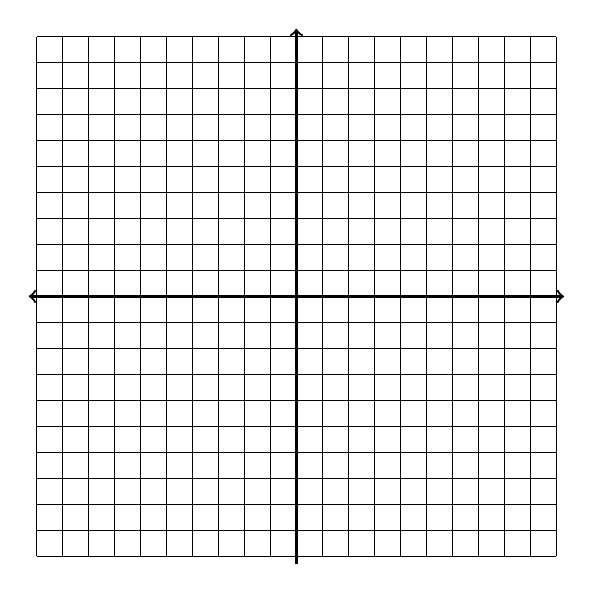
\begin{tikzpicture}[xscale=0.33,yscale=0.33]
	\draw [thick, <->] (-10.3,0) -- (10.3,0);
	\draw [thick, ->] (0,-10.3) -- (0,10.3);
	\draw [thin] (-10,-10) grid (10,10);
\end{tikzpicture}
\begin{exercises}{sec:0401p}

\lab{} On the grid above, graph $f(x)= \frac{1}{4}x^2$.

\lab{}  Applying transformational thinking, graph $y=f(x)-1$.

\lab{}  Absolute values ``flip'' some numbers and leave others untouched.  If we applied absolute values to the output ($y$), what part of the graph would be effected?  Circle or highlight that portion of your second graph.

\noindent
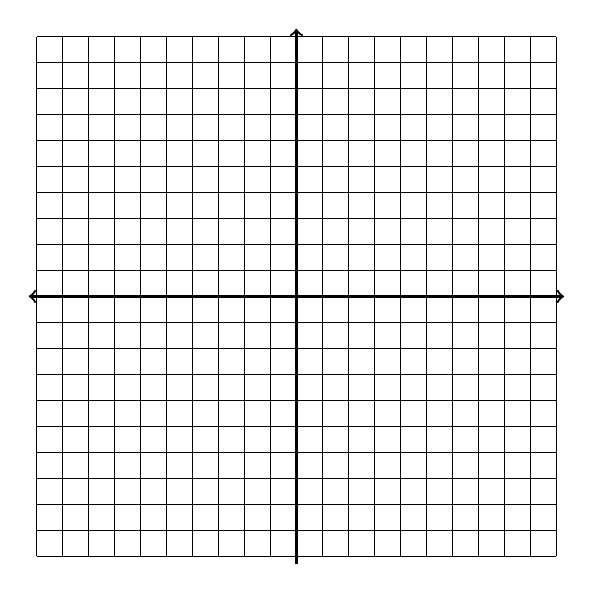
\begin{tikzpicture}[xscale=0.33,yscale=0.33]
	\draw [thick, <->] (-10.3,0) -- (10.3,0);
	\draw [thick, ->] (0,-10.3) -- (0,10.3);
	\draw [thin] (-10,-10) grid (10,10);
\end{tikzpicture}

\lab{}  On the grid above, graph $y=|f(x)-1|$.

\lab{}  What are the coordinates of the two cusps we have made?

\vspace{2cm}
\lab{}  Transform the previous graph by shifting it down 3 units.  What is the equation of this new function?

\vspace{2cm}
\lab{}  Name the three lattice points that will be effected if we applied absolute values to this equation.

\vspace{2cm}
\lab{}  Graph $x^3-3x-2$ as $Y_1$.  Draw it below.

\noindent
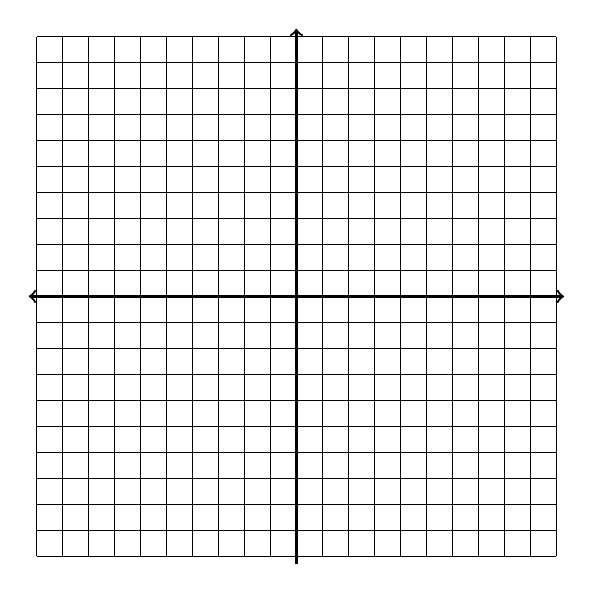
\begin{tikzpicture}[xscale=0.33,yscale=0.33]
	\draw [thick, <->] (-10.3,0) -- (10.3,0);
	\draw [thick, ->] (0,-10.3) -- (0,10.3);
	\draw [thin] (-10,-10) grid (10,10);
\end{tikzpicture}

\lab{}  What do you anticipate $Y_2=Y_1(|X|)$ will look like?

\vspace{2cm}
\lab{}  Verify in your TI-8*.  Describe what the absolute value did to the graph.


\vspace{2cm}
\lab{} How are absolute values differ if applied before vs. after?


\end{exercises}
\end{multicols*}